\documentclass[a4paper,twoside]{article}
\usepackage[T1]{fontenc}
\usepackage[bahasa]{babel}
\usepackage{graphicx}
\usepackage{graphics}
\graphicspath{ {./gambar/} }
\usepackage{float}
\usepackage[cm]{fullpage}
\pagestyle{myheadings}
\usepackage{etoolbox}
\usepackage{setspace} 
\usepackage{lipsum} 
\setlength{\headsep}{30pt}
\usepackage[inner=2cm,outer=2.5cm,top=2.5cm,bottom=2cm]{geometry} %margin
% \pagestyle{empty}

\makeatletter
\renewcommand{\@maketitle} {\begin{center} {\LARGE \textbf{ \textsc{\@title}} \par} \bigskip {\large \textbf{\textsc{\@author}} }\end{center} }
\renewcommand{\thispagestyle}[1]{}
\markright{\textbf{\textsc{AIF184001 \textemdash Rencana Kerja Skripsi \textemdash Sem. Ganjil 2019/2020}}}

\newcommand{\HRule}{\rule{\linewidth}{0.4mm}}
\renewcommand{\baselinestretch}{1}
\setlength{\parindent}{0 pt}
\setlength{\parskip}{6 pt}

\onehalfspacing
 
\begin{document}

\title{\@judultopik}
\author{\nama \textendash \@npm} 

%tulis nama dan NPM anda di sini:
\newcommand{\nama}{Hapsari Laksmi W}
\newcommand{\@npm}{2015730037}
\newcommand{\@judultopik}{Migrasi \textit{Zurb Foundation} ke \textit{Bootstrap 4}} % Judul/topik anda
\newcommand{\jumpemb}{1} % Jumlah pembimbing, 1 atau 2
\newcommand{\tanggal}{24/08/2019}

% Dokumen hasil template ini harus dicetak bolak-balik !!!!

\maketitle

\pagenumbering{arabic}

\section{Deskripsi}
%Tuliskan deskripsi dari topik skripsi yang akan anda ajukan. Di sini dapat dituliskan latar belakang, seperti apa penelitian yang sudah ada sebelumnya dan apa yang akan anda kerjakan. Sertakan gambar agar penjelasan anda menjadi lebih baik.

BlueTape merupakan aplikasi berbasis \textit{web} yang berfungsi mengolah beberapa kebutuhan administrasi fakultas secara \textit{paperless} yang digunakan dalam lingkungan FTIS UNPAR.  Aplikasi ini mempunyai fitur untuk manajemen transkrip nilai, perubahan kuliah dan jadwal dosen. \textit{Framework} yang digunakan dalam aplikasi BlueTape ada dua yaitu \textit{Codeigniter} dan \textit{Zurb Foundation}.  

\begin{figure}[h]
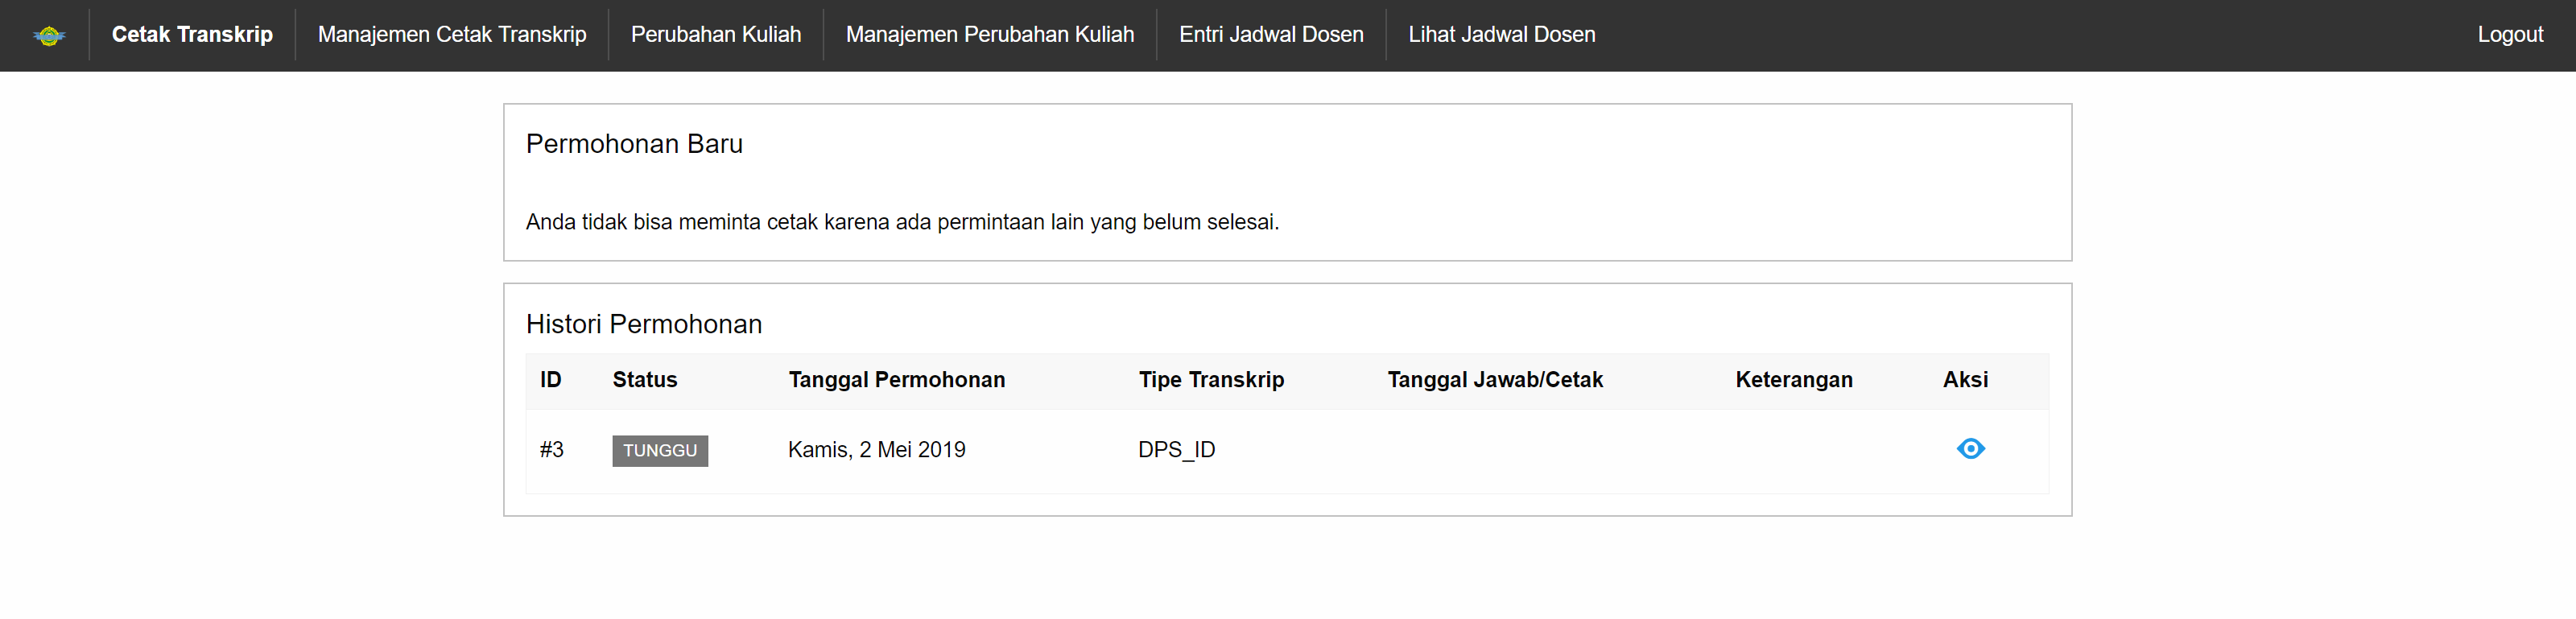
\includegraphics [scale=0.5] {Tampilan-Cetak-Transkrip.PNG}
\caption{Tampilan Cetak Transkrip}
\end{figure}

\begin{figure}[h]
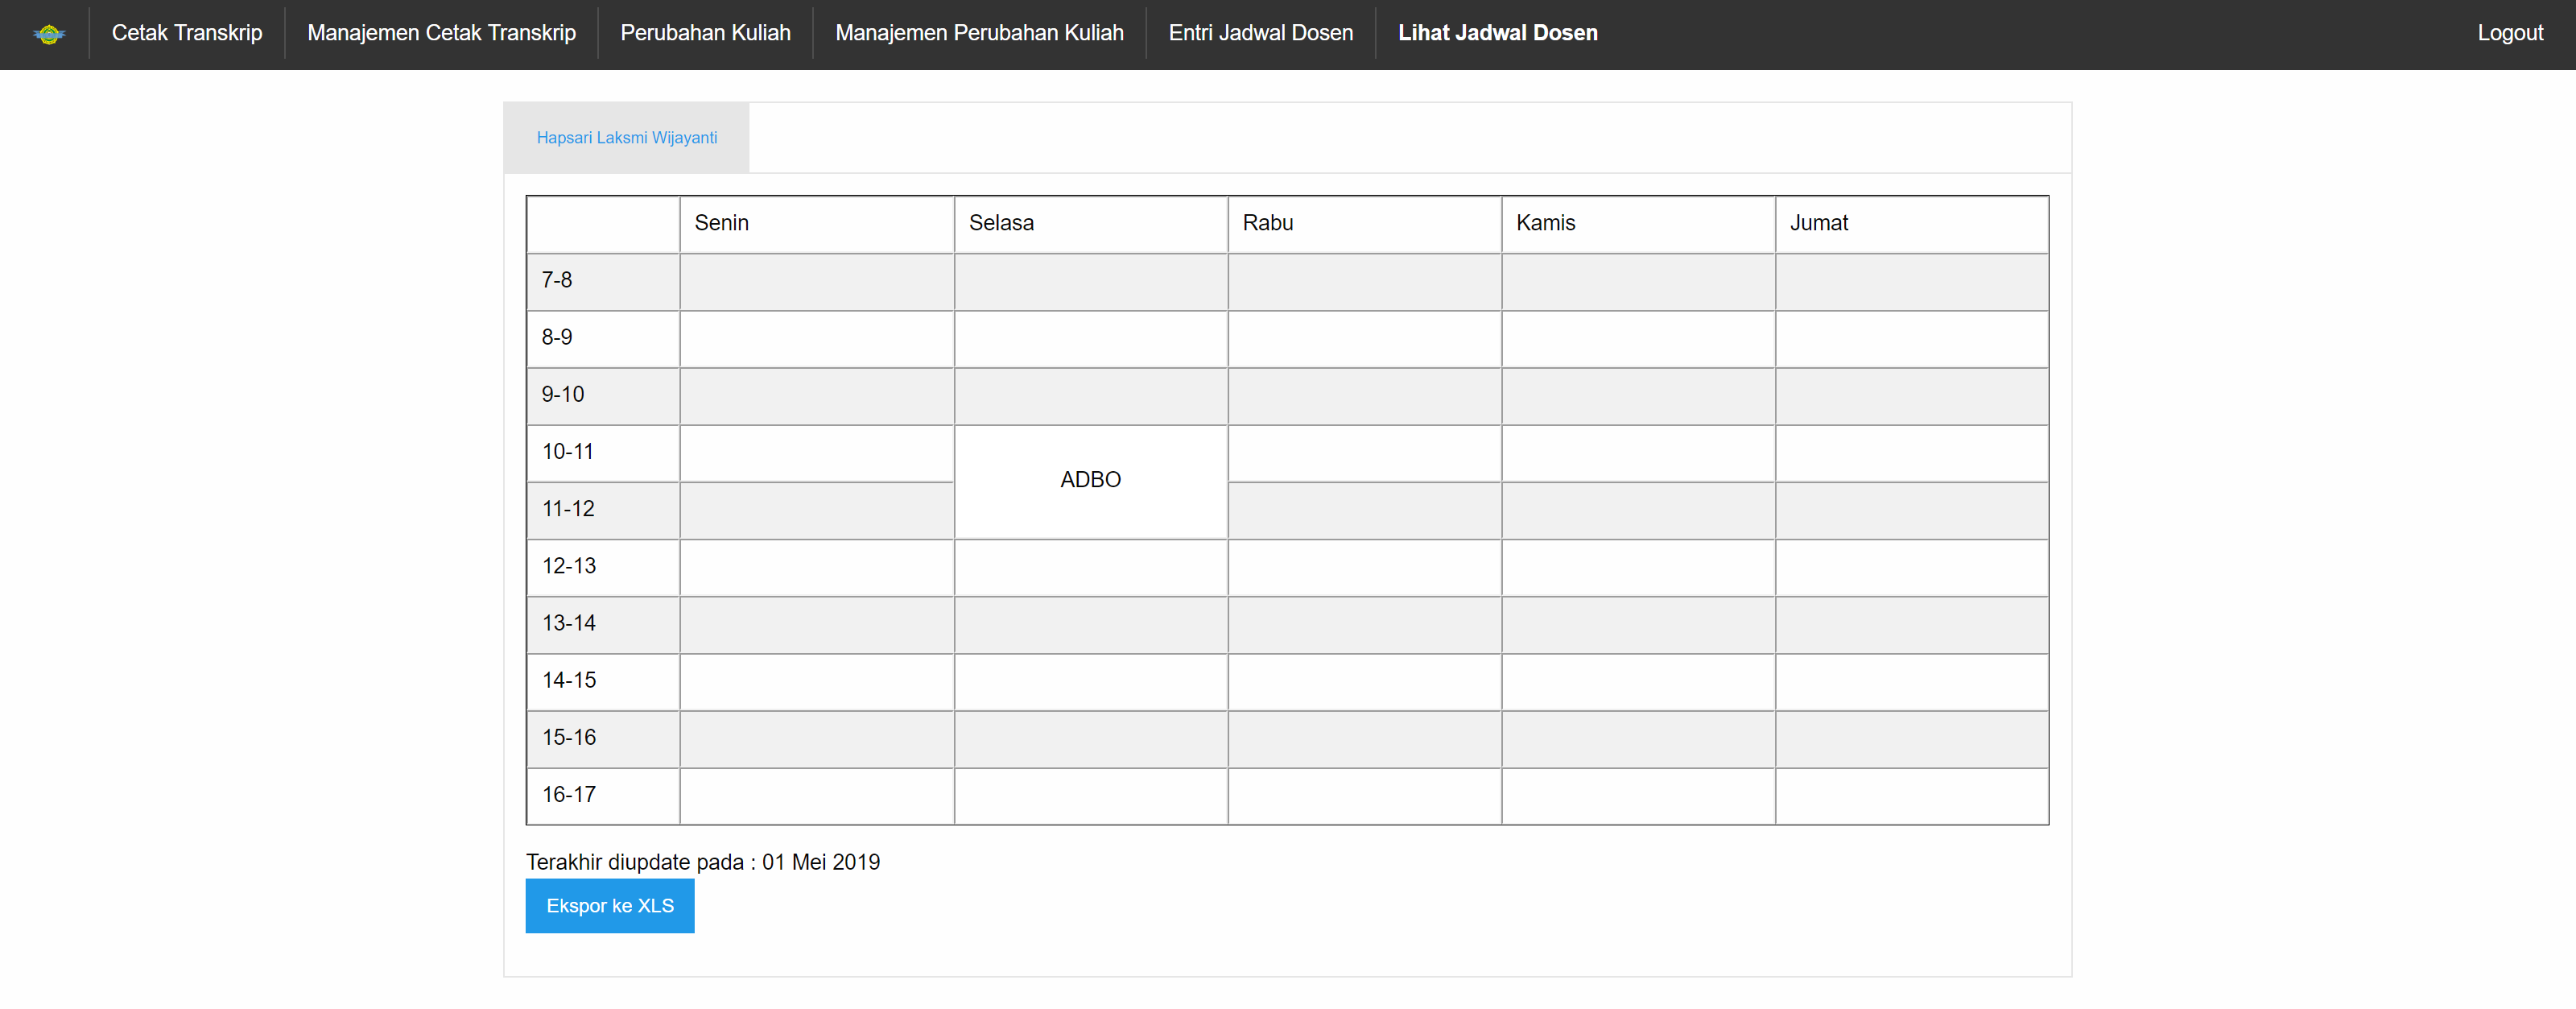
\includegraphics [scale=0.5] {Tampilan-Lihat-Jadwal-Dosen.PNG}
\caption{Tampilan Lihat Jadwal Dosen}
\end{figure}

\begin{figure}[h]
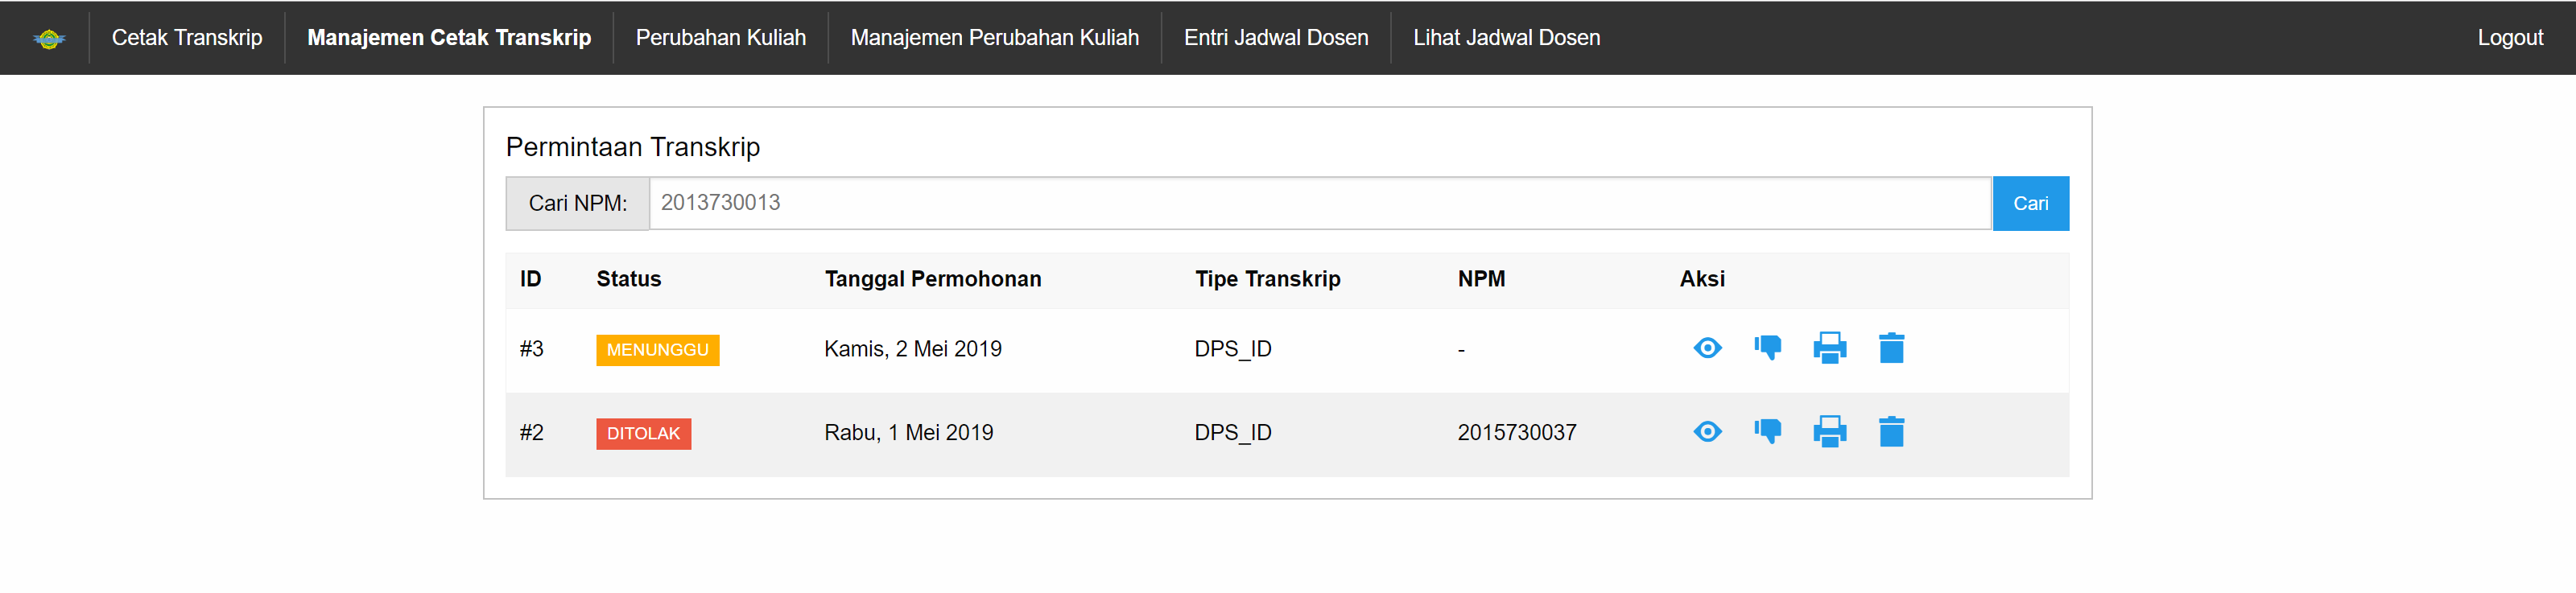
\includegraphics [scale=0.5] {Tampilan-Manajemen-Cetak-Transkrip.PNG}
\caption{Tampilan-Manajemen-Cetak-Transkrip}
\end{figure}

\begin{figure}[h]
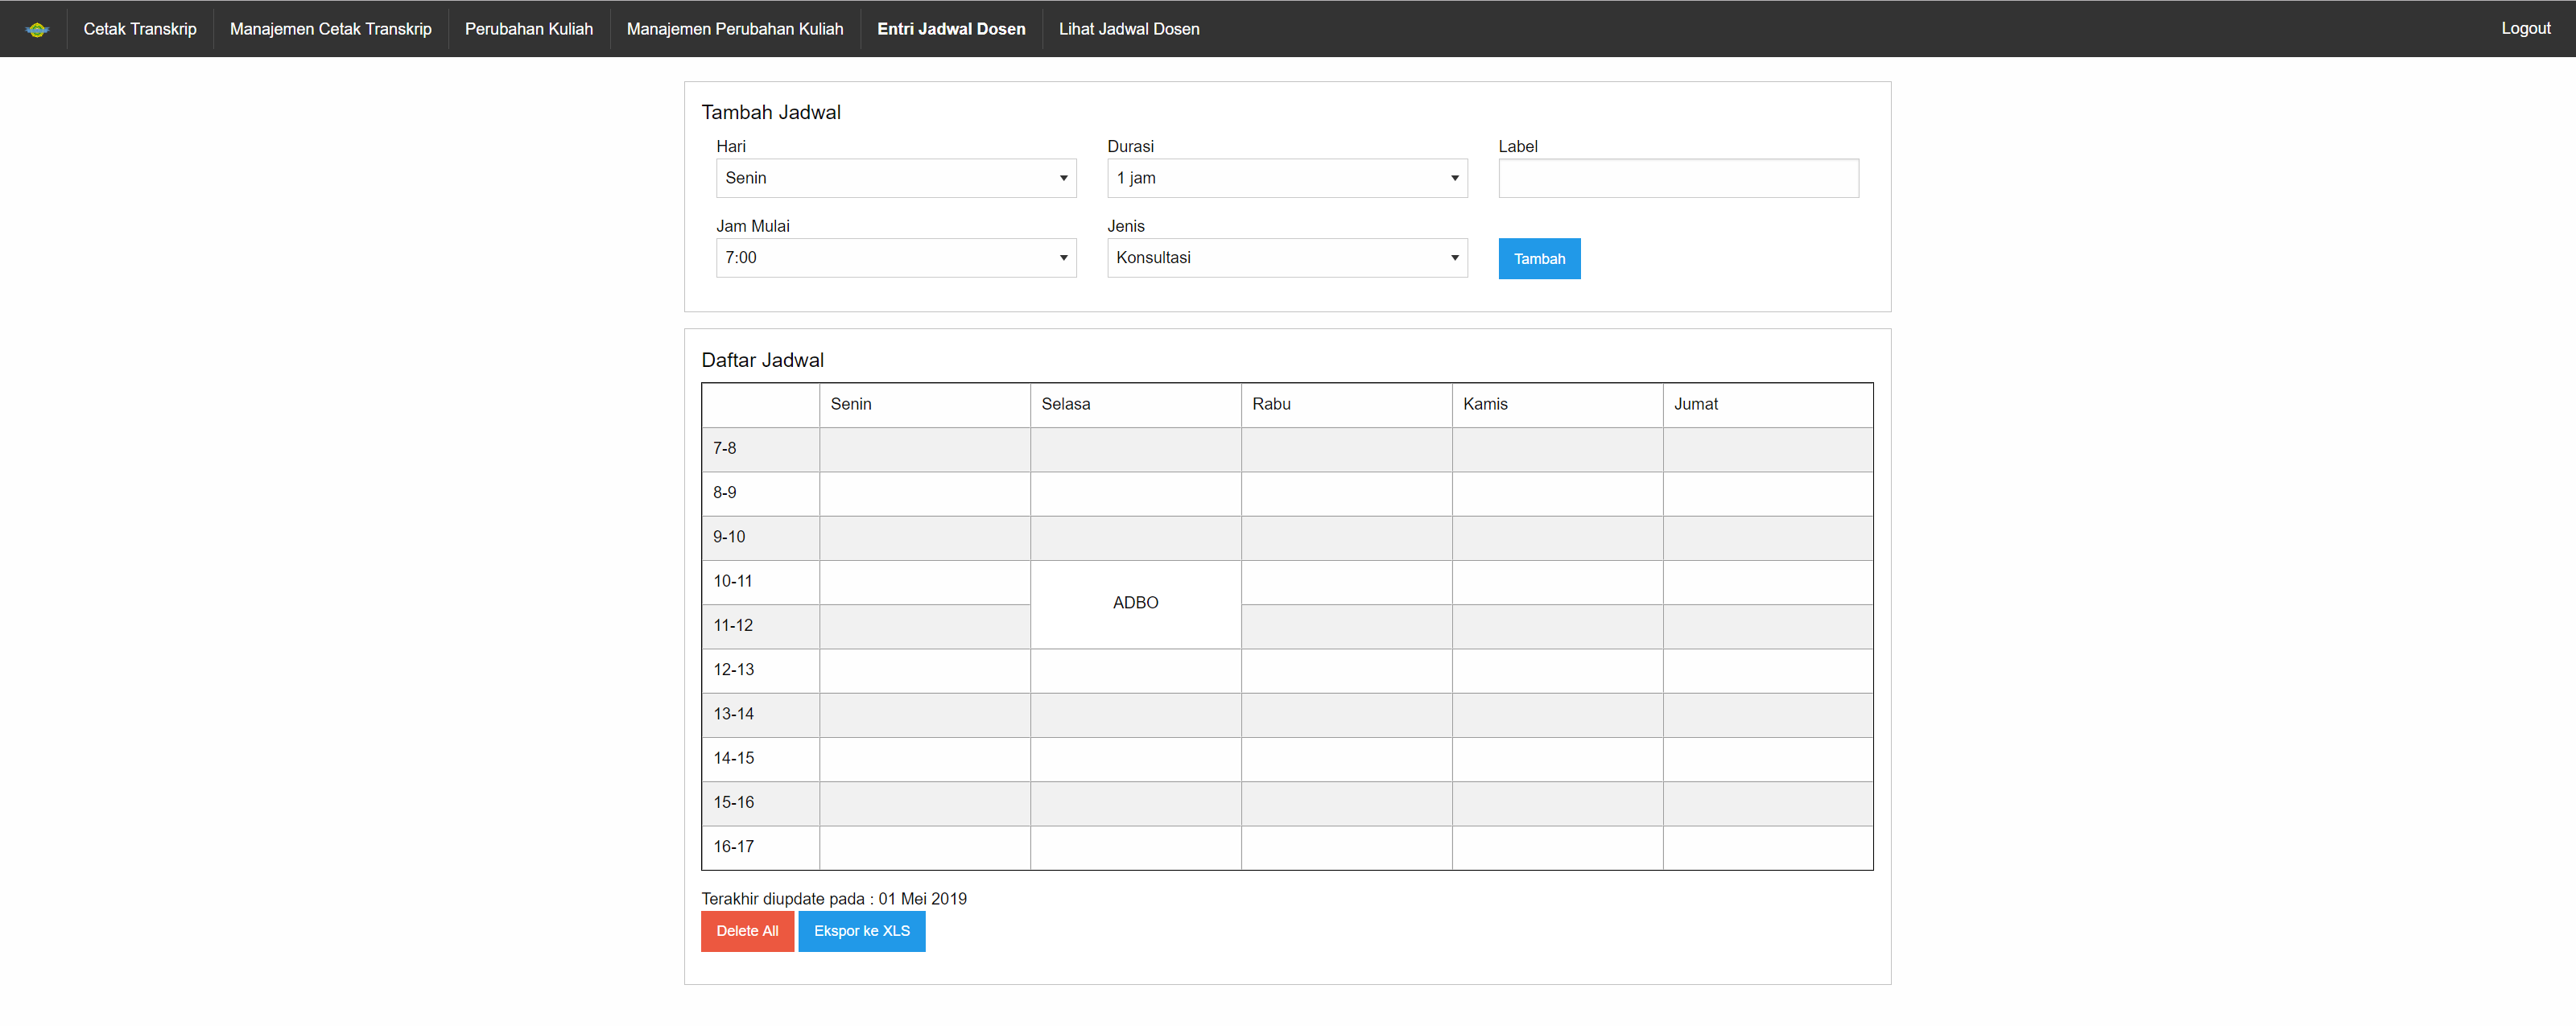
\includegraphics [scale=0.5] {Tampilan-Entri-Jadwal-Dosen.PNG}
\caption{Tampilan Entri Jadwal Dosen}
\end{figure}

\begin{figure}[h]
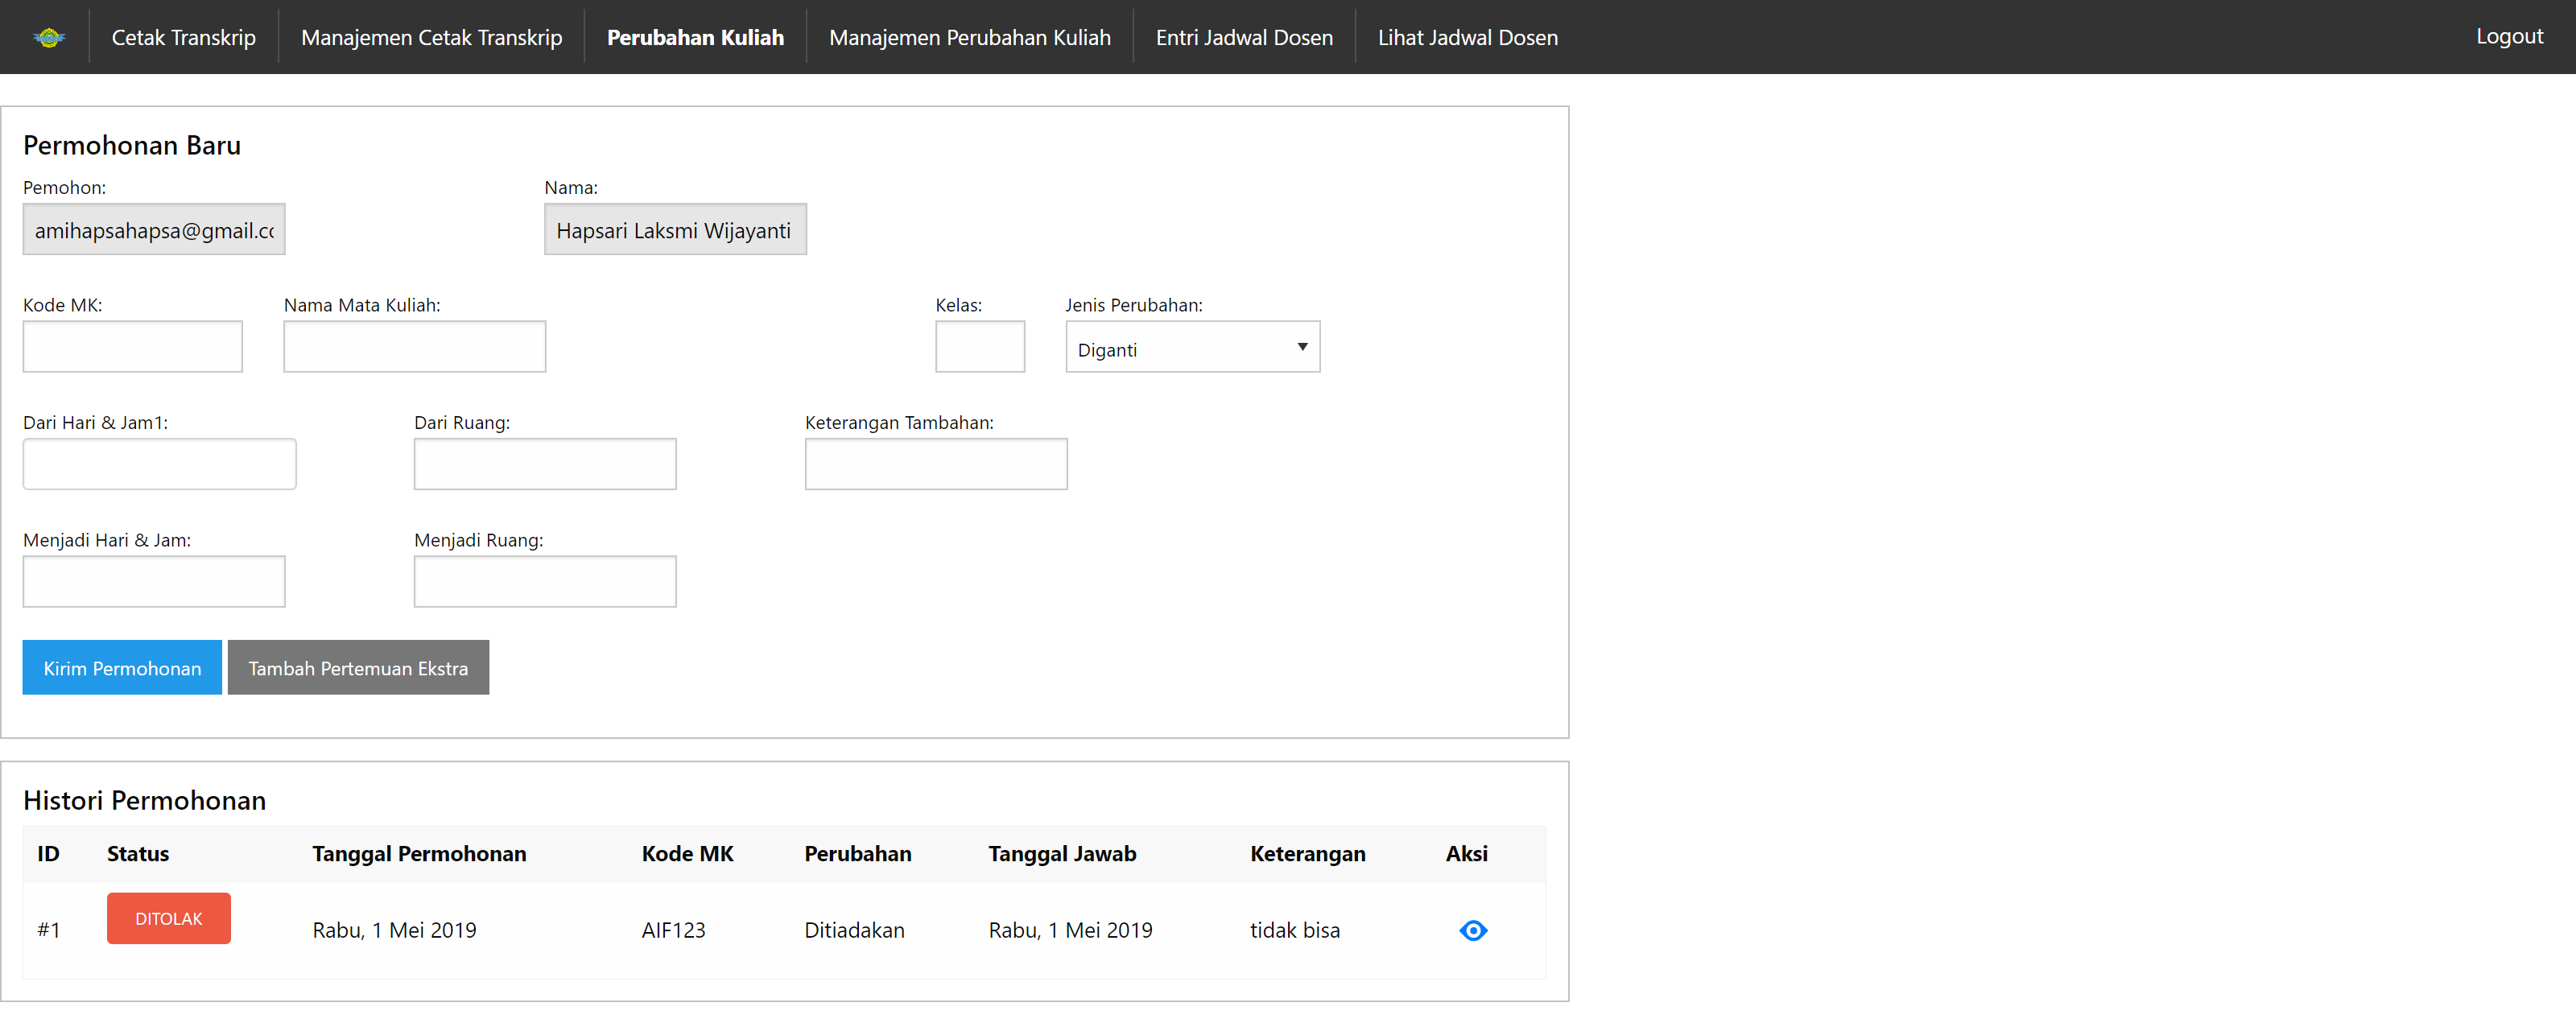
\includegraphics [scale=0.5] {Tampilan-Perubahan-Kuliah.PNG}
\caption{Tampilan Perubahan Kuliah}
\end{figure}

\begin{figure}[h!]
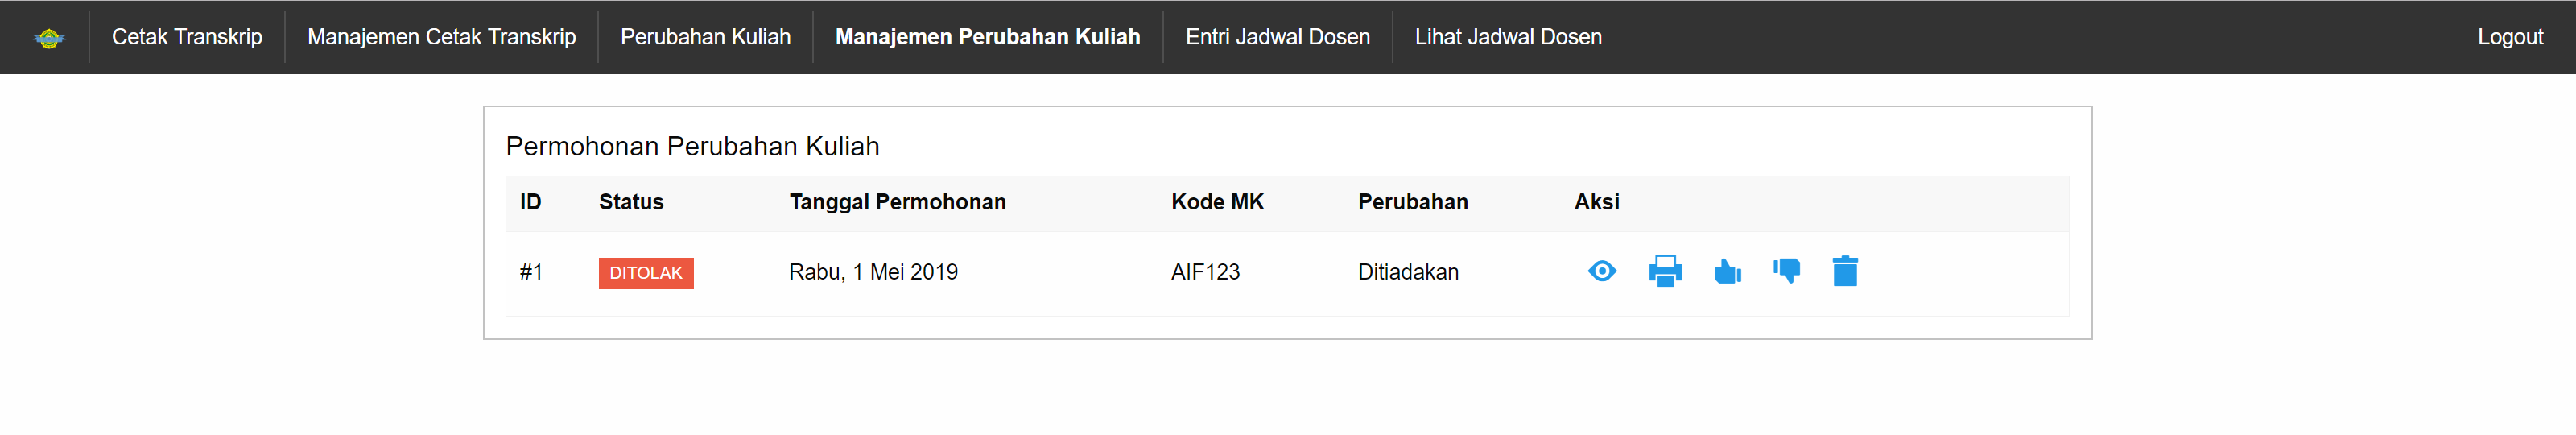
\includegraphics [scale=0.5] {Tampilan-Manajemen-Perubahan-Kuliah.PNG}
\caption{Tampilan Manajemen Perubahan Kuliah}
\end{figure}




Meskipun \textit{open-source}, saat ini \textit{Zurb Foundation} tidak sepopuler \textit{framework} \textit{Bootstrap}. 
\textit{Bootstrap} adalah \textit{ Javascript framework} yang didesain untuk membantu membangun komponen \textit{user interface} yang terdiri dari \textit{CSS, JavaScript/jQuery}, dan \textit{glyphicons}. Pembangunan \textit{website} yang lebih cepat dan besarnya komunitas yang ada berdampak pada banyaknya pengembang \textit{web} yang memanfaatkan \textit{framework Bootstrap}. Sehingga jumlah proyek yang dihasilkan oleh\textit{ framework Bootstrap} lebih banyak dibanding \textit{Zurb Foundation}. 

%Pada skripsi ini, akan dibuat sebuah perangkat lunak yang dapat menampilkan visualisasi dan simulasi kerumunan orang yang berkunjung ke sebuah museum. Dengan menggunakan perangkat lunak tersebut, pengelola museum dapat mengatur tempat peletakan objek sehingga tidak terjadi kerumunan yang terlalu padat.
%

%Dari berbagai macam teknik yang dapat digunakan untuk melakukan simulasi kerumunan, dipilih dua buah teknik yaitu teknik {\it flow tiles} dan {\it social force model (steering behaviour)}.
%
%Dst, dst, dst, \ldots\ldots\ldots 
%
%Perangkat lunak akan dibuat dengan bantuan {\it framework} OpenSteer. Sebagai studi kasus, museum yang digunakan untuk melakukan simulasi adalah Museum Geologi Bandung.
%
%Dst, dst, dst, \ldots\ldots\ldots 
Pada skripsi ini akan dirubah \textit{view} pada keseluruhan  aplikasi BlueTape menggunakan \textit{framework} Bootstrap 4. Setiap view menggunakan template yang menampilkan nama \textit{module}, menu navigasi, dan \textit{flash message} (bila diperlukan).



\section{Rumusan Masalah}
%Tuliskan rumusan dari masalah yang akan anda bahas pada skripsi ini. Rumusan masalah biasanya berupa kalimat pertanyaan. Gunakan itemize seperti contoh di bagian Deskripsi Perangkat Lunak.

\begin{itemize}
	\item Bagaimana membuat \textit{template} manajemen cetak transkrip, manajemen perubahan kuliah dan manajemen jadwal dosen.
	\item Bagaimana mengimplentasikan \textit{plugin} yang tersedia di dalam \textit{Bootstrap 4}.
\end{itemize}

\section{Tujuan}
%Tuliskan tujuan dari topik skripsi yang anda ajukan. Tujuan penelitian biasanya berkaitan erat dengan pertanyaan yang diajukan di bagian rumusan masalah. Gunakan itemize seperti contoh di bagian Deskripsi Perangkat Lunak.
Tujuan yang ingin dicapai dalam penelitian ini :

	\begin{itemize}	
	\item Membuat \textit{template} cetak transkrip nilai, \textit{template} manajemen cetak transkrip, \textit{template} perubahan kuliah, \textit{module} manajemen perubahan kuliah, \textit{modul} entri jadwal dosen dan \textit{module} lihat jadwal dosen dengan \textit{framework Bootstrap 4} yang \textit{responsive} untuk berbagai platform.
	\item Mengimplentasikan \textit{plugin} yang tersedia dalam \textit{library} Bootstrap 4.
	
		
\end{itemize}
	
		


\section{Deskripsi Perangkat Lunak}

Perangkat lunak akhir yang akan dibuat memiliki fitur minimal sebagai berikut:
\begin{itemize}
	\item Mampu menghasilkan \textit{view}\textit{website} yang \textit{responsive} untuk berbagai \textit{platform} menggunakan \textit{Bootstrap 4}.
	\item Mampu mengimplementasikan \textit{plugin Bootstrap 4} sesuai kebutuhan aplikasi BlueTape	
		
\end{itemize}

\section{Detail Pengerjaan Skripsi}
Tuliskan bagian-bagian pengerjaan skripsi secara detail. Bagian pekerjaan tersebut mencakup awal hingga akhir skripsi, termasuk di dalamnya pengerjaan dokumentasi skripsi, pengujian, survei, dll.

Bagian-bagian pekerjaan skripsi ini adalah sebagai berikut :
	\begin{enumerate}
		\item Mempelajari \textit{framework PHP Codeigniter}.
		\item Mempelajari framework \textit{front-end} \textit{Bootstrap 4} beserta plugin-plugin yang tersedia
		\item Membuat rancangan tampilan website dan \textit{template}.
		\item Mengimplementasikan keseluruhan rancangan tampilan dan \textit{template}.
		\item Menulis dokumen skripsi.
	\end{enumerate}

\section{Rencana Kerja}
Rincian capaian yang direncanakan di Skripsi 1 adalah sebagai berikut:
\begin{enumerate}
\item Memahami penggunaan \textit{framework Bootstrap 4} dan \textit{CodeIgniter}, \textit{Zurb Foundation}.
\item Menganalisis plugin - plugin yang diperlukan dalam website Blue Tape.
\item Merancang tampilan \textit{website} Blue Tape menggunakan Bootstrap 4.
\item Menulis dokumen skripsi.
\end{enumerate}

Sedangkan yang akan diselesaikan di Skripsi 2 adalah sebagai berikut:
\begin{enumerate}
\item Mengimplementasi tampilan \textit{website} dengan \textit{Bootstrap 4}.
\item Menyelesaikan dokumen skripsi.
\end{enumerate}

\vspace{1cm}
\centering Bandung, \tanggal\\
\vspace{2cm} \nama \\ 
\vspace{1cm}

Menyetujui, \\
\ifdefstring{\jumpemb}{2}{
\vspace{1.5cm}
\begin{centering} Menyetujui,\\ \end{centering} \vspace{0.75cm}
\begin{minipage}[b]{0.45\linewidth}
% \centering Bandung, \makebox[0.5cm]{\hrulefill}/\makebox[0.5cm]{\hrulefill}/2013 \\
\vspace{2cm} Nama: \makebox[3cm]{\hrulefill}\\ Pembimbing Utama
\end{minipage} \hspace{0.5cm}
\begin{minipage}[b]{0.45\linewidth}
% \centering Bandung, \makebox[0.5cm]{\hrulefill}/\makebox[0.5cm]{\hrulefill}/2013\\
\vspace{2cm} Nama: \makebox[3cm]{\hrulefill}\\ Pembimbing Pendamping
\end{minipage}
\vspace{0.5cm}
}{
% \centering Bandung, \makebox[0.5cm]{\hrulefill}/\makebox[0.5cm]{\hrulefill}/2013\\
\vspace{2cm} Nama: \makebox[3cm]{\hrulefill}\\ Pembimbing Tunggal
}
\end{document}

